\documentclass[letterpaper]{report}
\usepackage[utf8]{inputenc}
\usepackage[spanish]{babel}
\usepackage{graphicx, float, subcaption, anysize, xcolor, listings}

\marginsize{1.5cm}{2cm}{1.5cm}{2cm}
\parindent = 0mm

%Definición de colores
\definecolor{codegreen}{rgb}{1,0,0}
\definecolor{codegray}{rgb}{0.5,0.5,0.5}
\definecolor{codepurple}{rgb}{0.58,0,0.82}
\definecolor{backcolour}{rgb}{0.95,0.95,0.92}

%Estilo de la impresión del código
\lstdefinestyle{mystyle}{
    backgroundcolor=\color{backcolour},   
    commentstyle=\color{codegreen},
    keywordstyle=\color{magenta},
    numberstyle=\tiny\color{codegray},
    stringstyle=\color{codepurple},
    basicstyle=\ttfamily\footnotesize,         
    breaklines=true, %Toma en cuenta los saltos de línea                 
    breakatwhitespace=false,
    captionpos=b, %Imprime el título abajo                                         
    numbers=left, %Código enumerado                    
    showtabs=false, %No muestra las tabulaciones                  
    showspaces=false,
    showstringspaces=false,
    tabsize=2 % Modificar la tabulación original del código
}
%Definición de caracteres para que sean impresos en el listing
\lstset{literate=
  {á}{{\'a}}1
  {é}{{\'e}}1
  {í}{{\'i}}1
  {ó}{{\'o}}1
  {ú}{{\'u}}1
  {Á}{{\'A}}1
  {É}{{\'E}}1
  {Í}{{\'I}}1
  {Ó}{{\'O}}1
  {Ú}{{\'U}}1
  {ñ}{{\~n}}1
  {ü}{{\"u}}1
  {Ü}{{\"U}}1
}
\lstset{style = mystyle}
%Cuerpo del reporte
\begin{document}

    \begin{figure}
        \subfloat{
\includegraphics[width=0.2\textwidth]{img/unamescudo}}
        \hfill
        \subfloat{
\includegraphics[width=0.2\textwidth]{img/escudofi_negro}}
    \end{figure}

    \begin{titlepage}
        \centering
        {\bfseries\LARGE UNIVERSIDAD NACIONAL AUT\'ONOMA DE M\'EXICO \par}
        \vspace{1cm}
        {\bfseries\LARGE FACULTAD DE INGENER\'IA \par}
        \vspace{1cm}
        {\bfseries\LARGE DIVISI\'ON DE INGENIER\'IA EL\'ECTRICA \par}
        \vspace{1cm}
        {\itshape\Large\textbf{Asignatura: Estructura y Programaci\'on de 
        Computadoras (1503)}}
        \vspace{1cm}
        {\itshape\Large\textbf{Proyecto 1: Compilador básico del MC68HC11}\par}
        \vspace{1cm}
        {\itshape\Large \textbf{Profesor: M.I Pedro Ignacio Rinc\'on G\'omez\\}
        \par}
        \vspace{1cm}
        \vfill
        {\itshape\Large \textbf{Integrantes del equipo:} \\\par}
        \begin{itemize}
            \centering
            {\itshape\Large
            \item [\textbullet] Bautista P\'erez Brian Jassiel
            \item [\textbullet] Calder\'on Guevara C\'esar Yair
            \item [\textbullet] Maceda Patricio Fernando
            \item [\textbullet] V\'azquez Flores Jos\'e Mart\'in}
        \end{itemize}
        \vfill
        \vspace{1cm}
        {\itshape\Large Fecha de entrega: \today\par}
    \end{titlepage}
    
    \section*{1. Identificaciones de los integrantes}
    
        \begin{figure}[h]
            \centering
            \begin{subfigure}{7cm}
                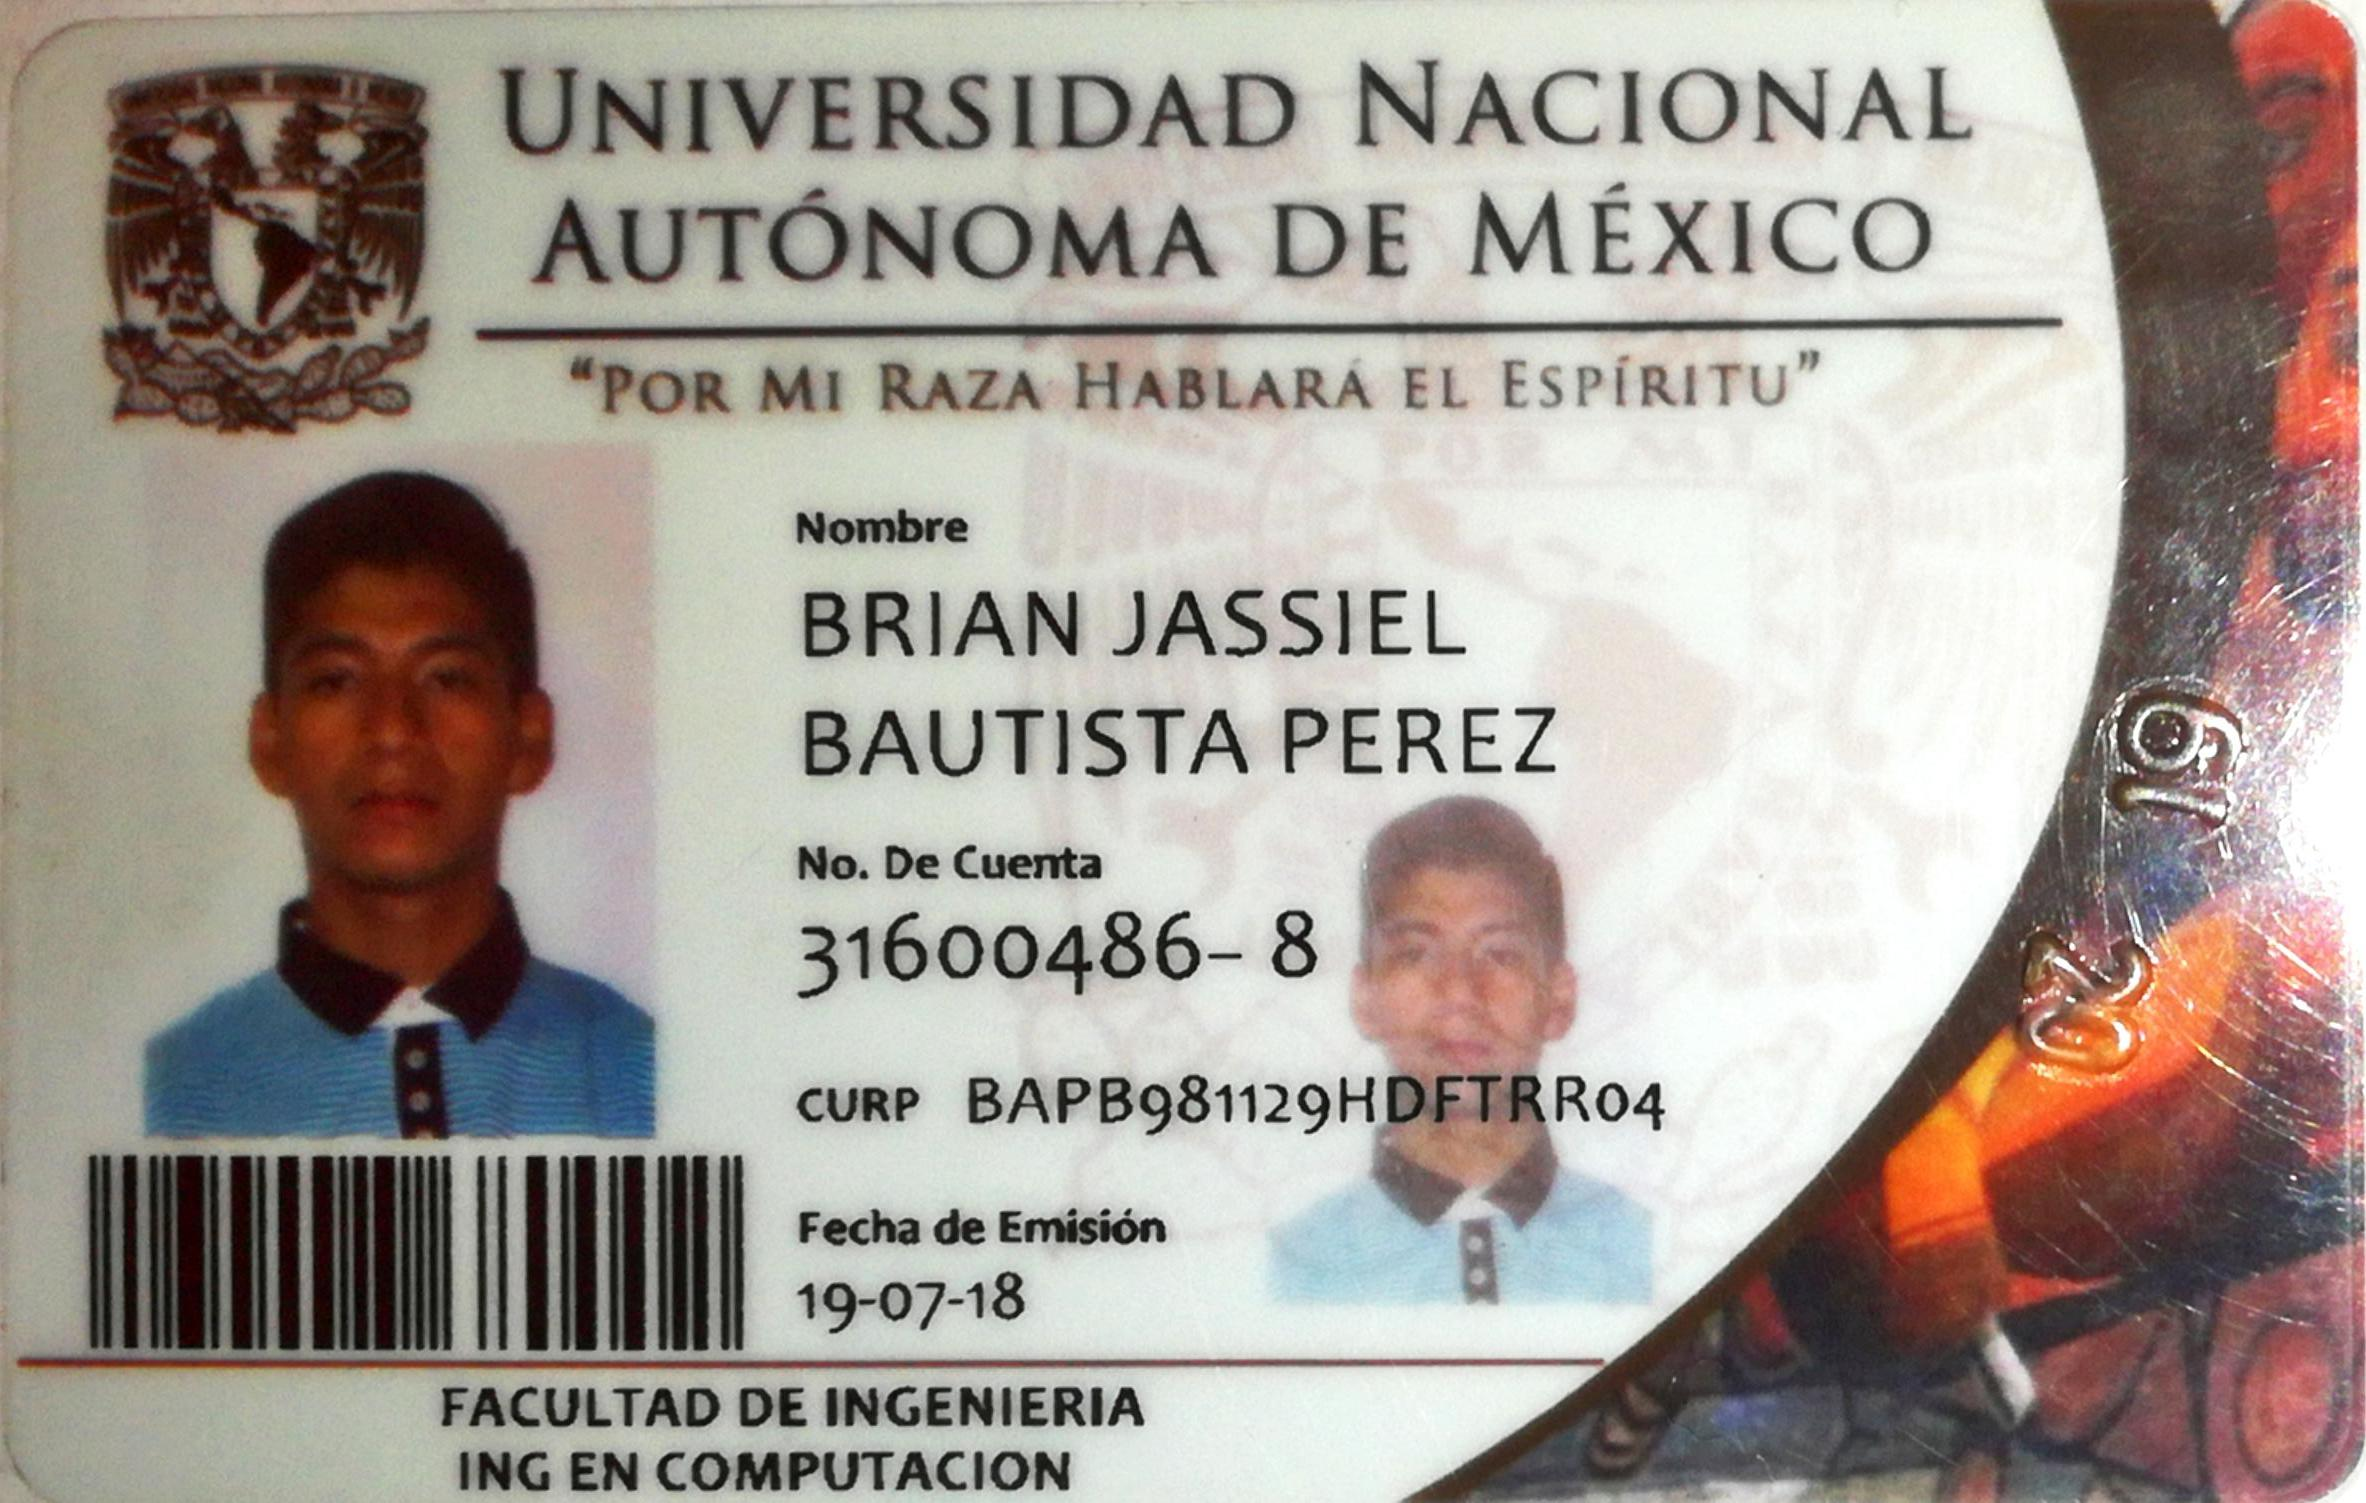
\includegraphics[width = 6cm]{img/Cr_Brian.jpg}
                \caption{Bautista P\'erez Brian Jassiel}
            \end{subfigure}
            \begin{subfigure}{7cm}
                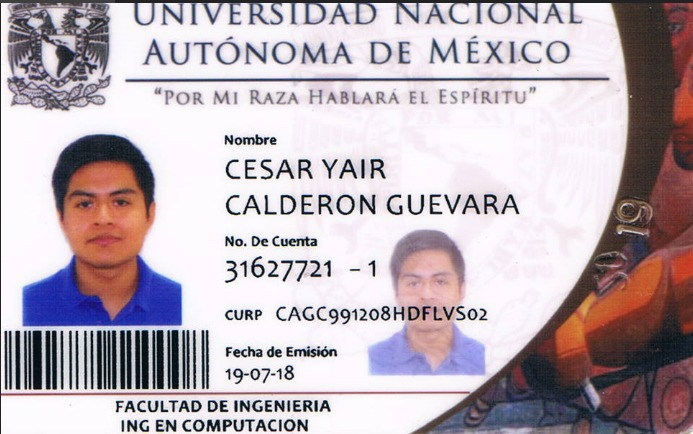
\includegraphics[width = 6cm]{img/Cr_Cesar}
                \caption{Calder\'on Guevara C\'esar Yair}
            \end{subfigure}
        \end{figure}
        \begin{figure}[h]
            \centering
            \begin{subfigure}{7cm}
                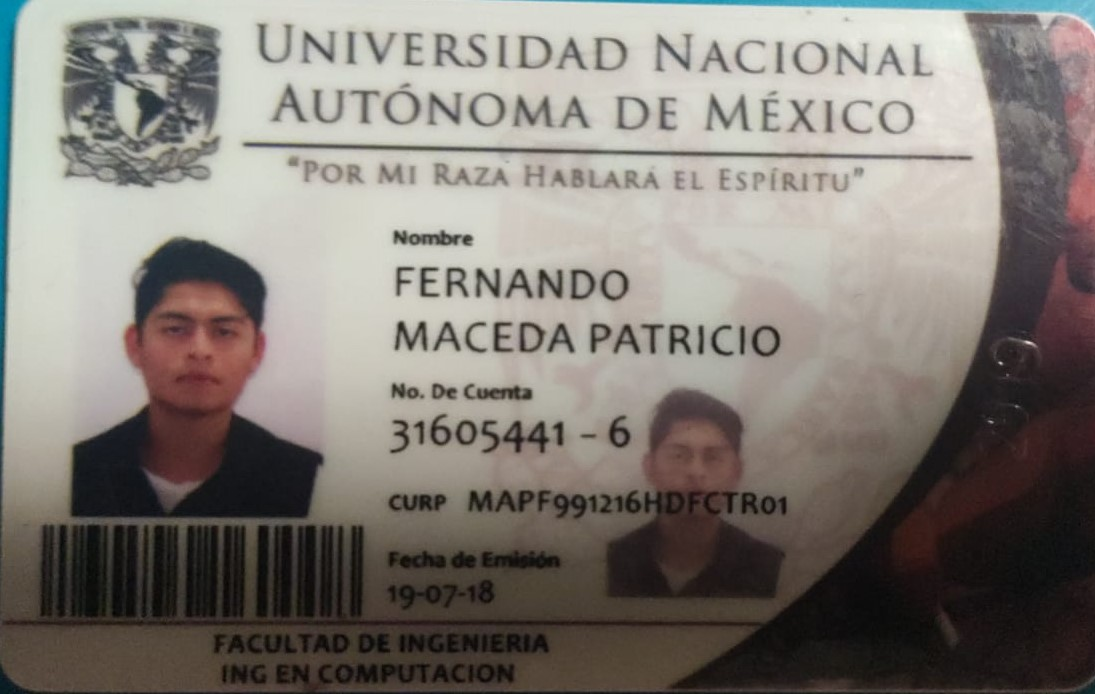
\includegraphics[width = 6cm]{img/Cr_Fer}
                \caption{Maceda Patricio Fernando}
            \end{subfigure}
            \begin{subfigure}{7cm}
                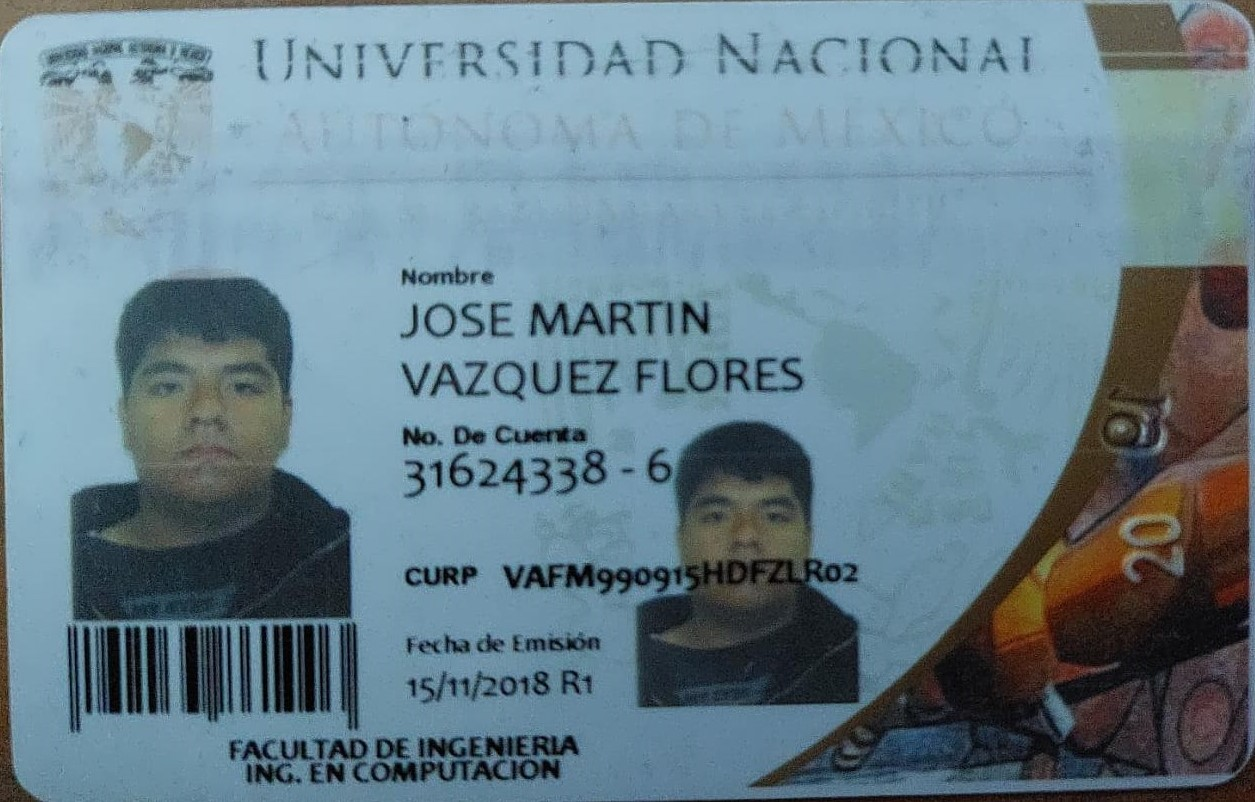
\includegraphics[width = 6cm]{img/Cr_Martin}
                \caption{V\'azquez Flores Jos\'e Mart\'in}
            \end{subfigure}
            \caption*{Integrantes del equipo que realiz\'o el proyecto.}
        \end{figure}

    \section*{2. Descripci\'on del proyecto y aportaciones}
    \subsection*{2.1 M\'odulo cient\'ifico pandas e importaciones}
    Tenemos la implemaci\'on del módulo \textbf{pandas} el cual nos servir\'a
    para leer el archivo de Excel en donde est\'an los comandos del MC68HC11.
    \lstinputlisting[language = Python, firstline = 1, lastline =2]
    {C:/Users/bjbp2/Documents/proyecto1_EyPC/MC68HC11.py}

    \subsection*{2.2 Funciones}
    En un principio tenemos la creación de 16 funciones (implementadas por el integrante 
    C\'esar Yair Calder\'on Guevara), las cuales en t\'erminos generales va a
    definir las operaciones del compilador del MC68HC11, a continuación daremos
    una breve explicaci\'on de lo que hace cada funci\'on.
    \begin{itemize}
        \item INICIO : Va a identificar la palabra reservada ORG y se marcar\'a el inicio del programa.
        \item fun\_cambio\_formato: Cambiará de formato decimal a hexadecimal.
        \item fun\_clr\_valor: Quita caracteres para el LST. 
        \item fun\_verifica\_long: Verifica que las variables y las palabras reservadas estén bien 
        escritas.
        \item fun\_verifica\_etiqueta: Verifica que las etiquetas estén escrita y añade sus valores.
        \item fun\_salto\_relativo: Verifica que el salto relativo no exceda los valores de memoria.
        \item ajuste\_De\_linea: Formatea las cadenas para que se ajusten los colores
        de impresi\'on
        \item quita\_comentarios:Quita las cadenas de palabras para generar el archivo que no contenga estos 
        comentarios.
        \item BNE : Verifica que el valor sea igual a cero para redireccionar a memoria.
        \item BRCLR : Si los bits valen cero, conduce a una operación.
        \item EQU : Asigna la etiqueta de valor dado para que pueda ser asignado.
        \item END : Marcamos el fin del programa.
        \item FCB : Genera un byte constante para agregar datos.
        \item JMP : Realizar los saltos en memoria a etiquetas dadas. 
        \item NOP : No realiza ninguna operaci\'on, lanza un error en caso de encontrar
         un valor.
        \item LDX : Cargar dato de 16 bits en el indice de X y en el indice de Y.
    \end{itemize}
    \lstinputlisting[language = Python, firstline = 10, lastline =240,
    caption = Implementac\'on de las funciones del compilador.]
    {C:/Users/bjbp2/Documents/proyecto1_EyPC/MC68HC11.py}

    \subsection*{2.3 Lectura del Excel}
    Esta sección del código (Implementada por los integrantes César y Brian Bautista) Tienen
    por objetivo la lectura del contenido del archivo Excel en el cual contiene
    los comandos y mnemonicos del MC68HC11. De este archivo se extraer\'an los comandos 
    según su OPCODE y para poder manipularlos, se guardar\'an en un diccionario según
    el tipo de direccionamiento al que cada comando pertenezca.

    \lstinputlisting[language = Python, firstline = 279, lastline =334,
    caption = Lectura del Excel y extracci\'on de datos.]
    {C:/Users/bjbp2/Documents/proyecto1_EyPC/MC68HC11.py}

    \subsection*{2.4 Implementaci\'on de clases}
    A continuaci\'on tenemos la creaci\'on de dos clases (Implementadas por el 
    integrante Fernando Maceda), la primera se va a encargar de indicar
    la cantidad de errores que contiene el programa en caso de que el c\'odigo
    se haya escrito de manera incorrecta, mientras que en la segunda clase se 
    definen una serie de variables y m\'etodos que se van a utilizar posteriormente.

    \lstinputlisting[language = Python, firstline = 246, lastline =271,
    caption = Implementac\'on de las clases.]
    {C:/Users/bjbp2/Documents/proyecto1_EyPC/MC68HC11.py}
    \subsection*{2.5 Excepciones para tratar con los errores del compilador}
    Como se ha visto en el paradigma de programaci\'on orientada a objetos, las
    excepciones tienen como prop\'osito el ejecutar el programa a\'un cuando un
    error se produjo durante la ejecuci\'on del programa.
    En este sentido, estas exepciones (Implementadas por el integrante Jos\'e 
    V\'azquez) van a marcar la cantidad de errores, no de este c\'odigo hecho en 
    \textbf{Python}, sino del c\'odigo que contiene el archivo ASC.
    Como en toda compilac\'on se leer\'a el archivo l\'inea por l\'inea y de haber
    errores, el compilador nos lo mostrar\'a. Para esto, antes de la verificaci\'on
    línea por línea y de las excepciones, se cre\'o un diccionario que contiene los
    mnemonicos del lenguaje del MC68HC11.

    \lstinputlisting[language = Python, firstline = 361, lastline = 397,
    caption = Diccionario de los mnemonicos.]
    {C:/Users/bjbp2/Documents/proyecto1_EyPC/MC68HC11.py}

    \lstinputlisting[language = Python, firstline = 399, lastline = 491,
    caption = Tratado de errores del compilador.]
    {C:/Users/bjbp2/Documents/proyecto1_EyPC/MC68HC11.py}

    \subsection*{2.6 Generación de los archivos
    que son producto de la compilación del archivo}

    Esta sección fue implementada por el integrante Brian Bautista. 
    En esta parte se generan los archivos LST y S19 una vez que el archivo ASC 
    fue compilado. Terminado este proceso se cierran los tres archivos y se le pide
    al usuario cerrar la ventana, pues si todo salió bien la compilación habrá
    finalizado.

    \lstinputlisting[language = Python, firstline = 595, lastline =606,
    caption = Generación de archivos.]
    {C:/Users/bjbp2/Documents/proyecto1_EyPC/MC68HC11.py}

    \subsection*{2.7 Ejecuci\'on del programa (Petici\'on del archivo ASC)}
    
    Esta parte del programa fue implementada por los integrantes Fernando Maceda
    y Jos\'e Vázquez. Es lo primero que realizará el programa antes de cualquier 
    cosa, la petición del archivo ASC el cual va a ser el que tiene nuestro código
    fuente y el que será compilado para después generar los archivos LST y S19.

    \lstinputlisting[language = Python, firstline = 339, lastline =359,
    caption = Ejecución del programa.]
    {C:/Users/bjbp2/Documents/proyecto1_EyPC/MC68HC11.py}

    \subsection*{2.7 Informe de la compilaci\'on y ubicaci\'on de los errores}
    
    En esta parte del programa, lo que se hará es que una vez que el archivo esté
    compilado, se mandarán a imprimir el número de errores en caso de haberlos y a su
    vez, la ubicación de la línea en la que se encontró el error.
    (Implementado por los integrantes César Guevara y Fernando Maceda)


    \lstinputlisting[language = Python, firstline = 497, lastline = 593,
    caption = Ubicación de los errores.]
    {C:/Users/bjbp2/Documents/proyecto1_EyPC/MC68HC11.py}
    
    \newpage
                
    \section*{3. Evidencias.}

    \begin{figure}[!ht]
        \centering
        \begin{subfigure}{10cm}
            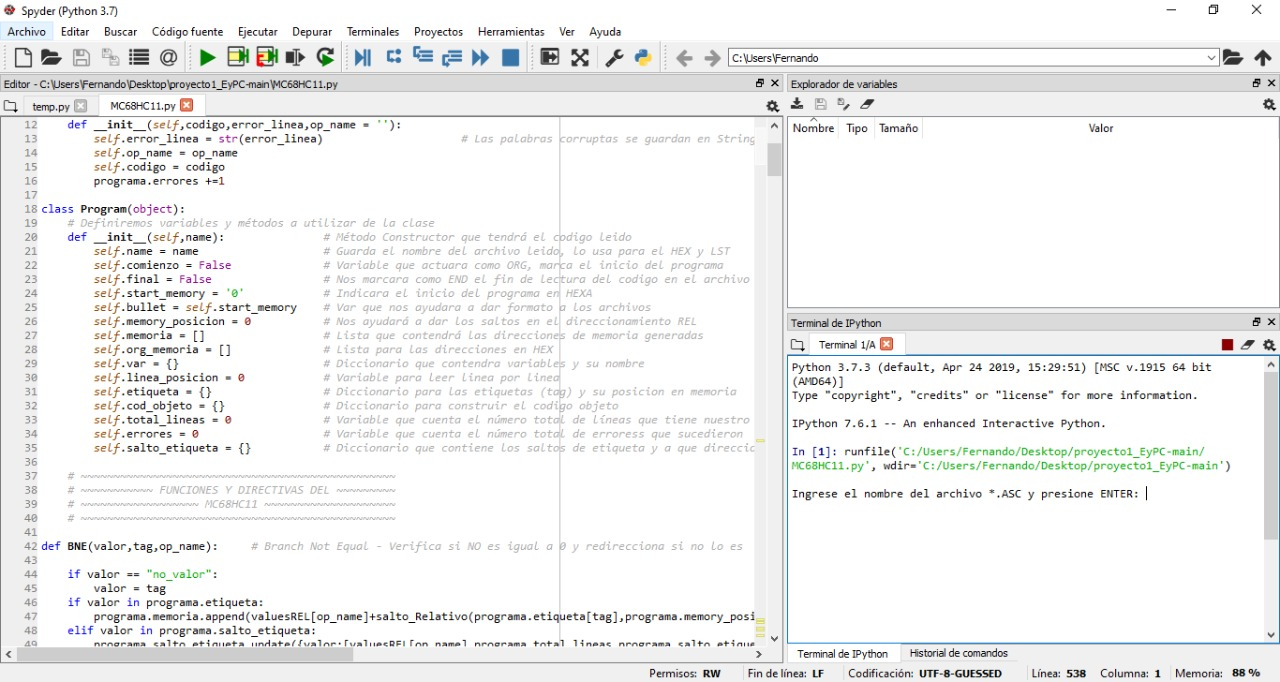
\includegraphics[width = 10cm]{img/E1}
            \caption{Programa en ejecución}
        \end{subfigure}
        \begin{subfigure}{10cm}
            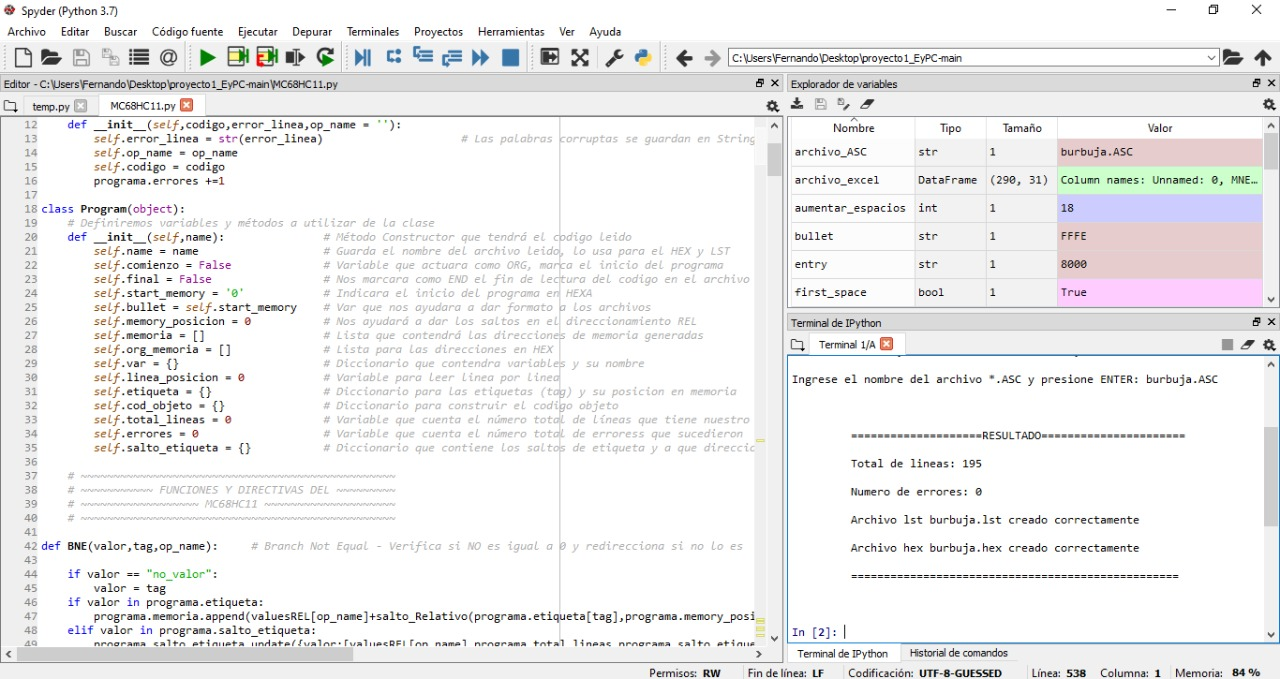
\includegraphics[width = 10cm]{img/E2}
            \caption{Programa compilado y arrojando los resultados}
        \end{subfigure}
        \begin{subfigure}{10cm}
            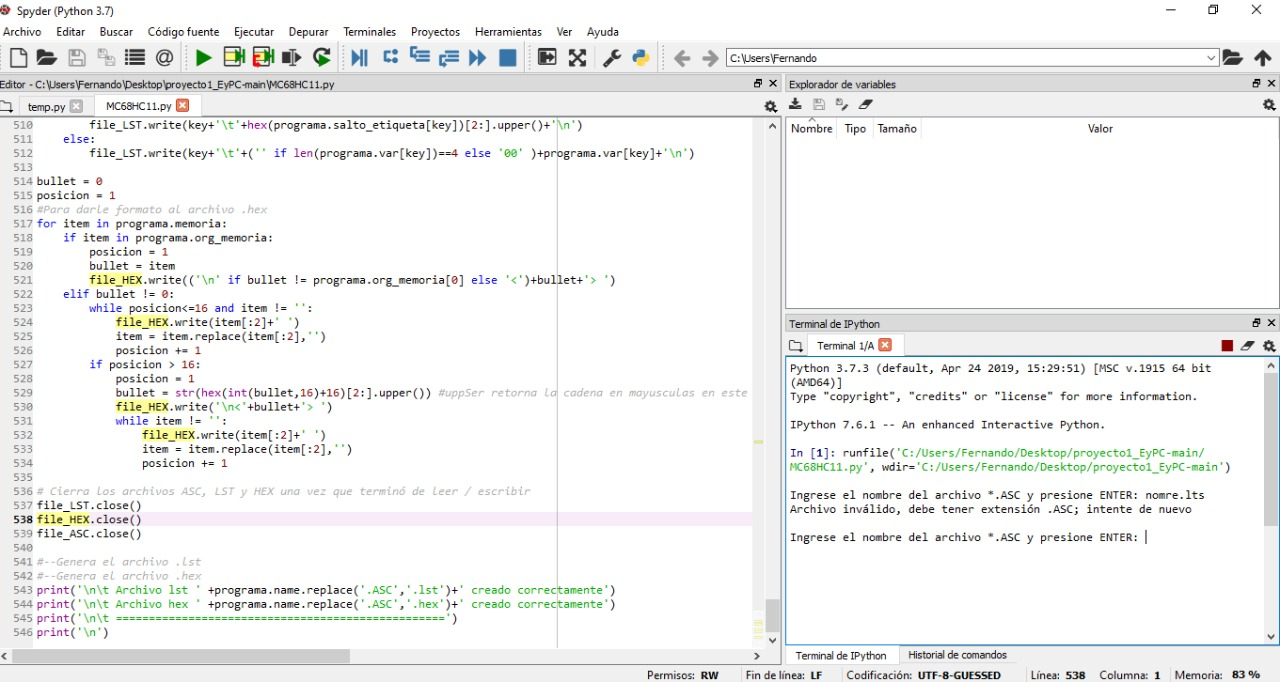
\includegraphics[width = 10cm]{img/E3}
            \caption{Error arrojado al no haber escrito correctamente el nombre
            del archivo ASC}
        \end{subfigure}
        \caption{Evidencias de ejecución del compilador del MC68HC11}
    \end{figure}
\end{document}